% Source: graduate-coursework/Prior_Semesters/Sp24/EMCH354/assignments/HW2/HW2.tex

\documentclass[border=4pt]{standalone}
\usepackage{amsmath}
\usepackage{tikz}
\usetikzlibrary{patterns}
\usetikzlibrary{arrows.meta, decorations.pathmorphing}

\definecolor{bluecolor}{RGB}{173,216,230}
\definecolor{purplecolor}{RGB}{210,180,222}
\definecolor{pinkcolor}{RGB}{255,182,193}
\definecolor{orangecolor}{RGB}{252, 213, 180}

\begin{document}
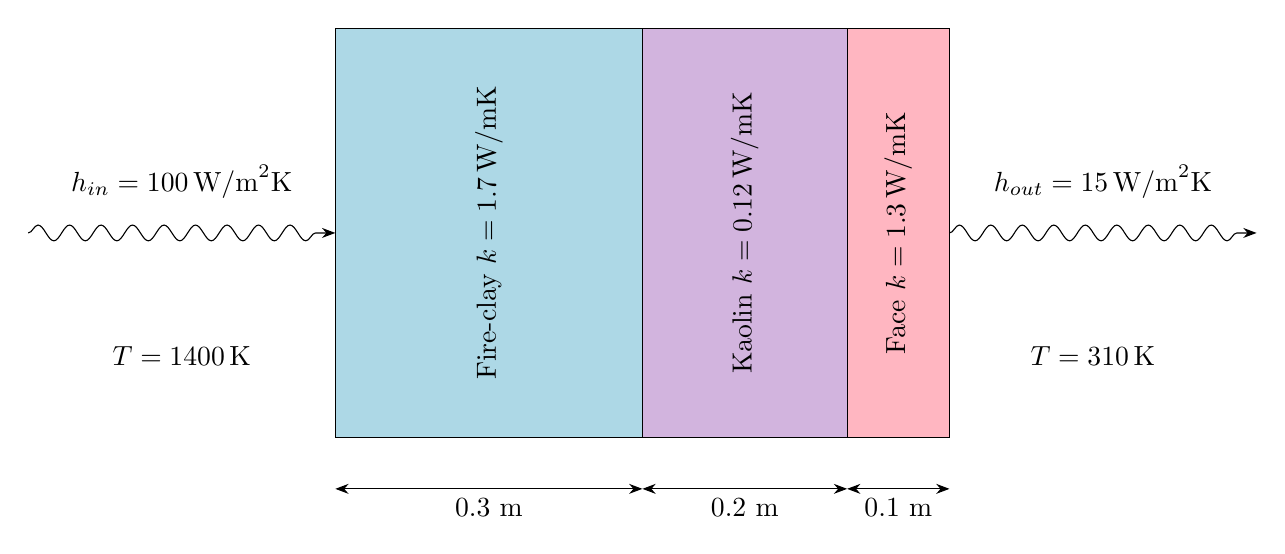
\begin{tikzpicture}[scale=1.3, >=Stealth]

% Define the layers with their thicknesses and thermal conductivities
\def\fireclay{3}
\def\kaolin{2}
\def\facebrick{1}
\def\wallheight{4}

% Fire-clay brick layer
\draw[fill=bluecolor] (0,0) rectangle (\fireclay,\wallheight) node[midway, rotate=90] {Fire-clay $k=1.7 \, \text{W/mK}$};

% Kaolin brick layer
\draw[fill=purplecolor] (\fireclay,0) rectangle (\fireclay+\kaolin,\wallheight) node[midway, rotate=90] {Kaolin $k=0.12 \, \text{W/mK}$};

% Face brick layer
\draw[fill=pinkcolor] (\fireclay+\kaolin,0) rectangle (\fireclay+\kaolin+\facebrick,\wallheight) node[midway, rotate=90] {Face $k=1.3 \, \text{W/mK}$};

% Inside heat transfer coefficient
\draw[->, decorate, decoration={snake, amplitude=1mm, segment length=4mm, post length=1mm}] (-3,\wallheight/2) -- (0,\wallheight/2);
\node at (-1.5,\wallheight/2+0.5) {$h_{in}=100 \, \text{W/m}^2\text{K}$};
\node at (-1.5,\wallheight/2-1.2) {$T=1400 \, \text{K}$} ;

% Outside heat transfer coefficient

% Wavy line
\draw[->, decorate, decoration={snake, amplitude=1mm, segment length=4mm, post length=1mm}] (6,\wallheight/2) -- (9,\wallheight/2);

\node at (7.5,\wallheight/2+0.5) {$h_{out}=15 \, \text{W/m}^2\text{K}$};
\node at (7.4,\wallheight/2-1.2) {$T=310 \, \text{K}$} ;
 
% Dimensions
\draw[<->] (0,-0.5) -- node[below] {0.3 m} (\fireclay,-0.5);
\draw[<->] (\fireclay,-0.5) -- node[below] {0.2 m} (\fireclay+\kaolin,-0.5);
\draw[<->] (\fireclay+\kaolin,-0.5) -- node[below] {0.1 m} (\fireclay+\kaolin+\facebrick,-0.5);

\end{tikzpicture}
\end{document}
